%----------------------------------------------------------------------------------------
%	PACKAGES AND THEMES
%----------------------------------------------------------------------------------------

\documentclass[table]{beamer}

\mode<presentation> {

% The Beamer class comes with a number of default slide themes
% which change the colors and layouts of slides. Below this is a list
% of all the themes, uncomment each in turn to see what they look like.

%\usetheme{default}
%\usetheme{AnnArbor}
%\usetheme{Antibes}
%\usetheme{Bergen}
%\usetheme{Berkeley}
%\usetheme{Berlin}
%\usetheme{Boadilla}
%\usetheme{CambridgeUS}
\usetheme{Copenhagen}
%\usetheme{Darmstadt}
%\usetheme{Dresden}
%\usetheme{Frankfurt}
%\usetheme{Goettingen}
%\usetheme{Hannover}
%\usetheme{Ilmenau}
%\usetheme{JuanLesPins}
%\usetheme{Luebeck}
%\usetheme{Madrid}
%\usetheme{Malmoe}
%\usetheme{Marburg}
%\usetheme{Montpellier}
%\usetheme{PaloAlto}
%\usetheme{Pittsburgh}
%\usetheme{Rochester}
%\usetheme{Singapore}
%\usetheme{Szeged}
%\usetheme{Warsaw}

% As well as themes, the Beamer class has a number of color themes
% for any slide theme. Uncomment each of these in turn to see how it
% changes the colors of your current slide theme.

%\usecolortheme{albatross}
%\usecolortheme{beaver}
%\usecolortheme{beetle}
%\usecolortheme{crane}
%\usecolortheme{dolphin}
%\usecolortheme{dove}
%\usecolortheme{fly}
%\usecolortheme{lily}
%\usecolortheme{orchid}
%\usecolortheme{rose}
%\usecolortheme{seagull}
%\usecolortheme{seahorse}
%\usecolortheme{whale}
%\usecolortheme{wolverine}

%\setbeamertemplate{footline} % To remove the footer line in all slides uncomment this line
%\setbeamertemplate{footline}[page number] % To replace the footer line in all slides with a simple slide count uncomment this line

%\setbeamertemplate{navigation symbols}{} % To remove the navigation symbols from the bottom of all slides uncomment this line
}

\usepackage{graphicx} % Allows including images
\usepackage{epstopdf}
\usepackage{booktabs} % Allows the use of \toprule, \midrule and \bottomrule in tables
\usepackage{multirow}
\usepackage[export]{adjustbox}
\usepackage{gensymb}
\renewcommand\footnoterule{{\color{black}\hrule height 0pt}}
\usepackage{appendixnumberbeamer} 
\usepackage{textgreek}
\usepackage{xcolor}
\usepackage{colortbl}
\usepackage{gensymb}
\graphicspath{{pics}}
\usepackage[normalem]{ulem}
\usepackage{mathtools}
\usepackage{amsmath}
\usepackage{amsfonts}

\newcommand{\overbar}[1]{\mkern 1.5mu\overline{\mkern-1.5mu#1\mkern-1.5mu}\mkern 1.5mu}

\setbeamertemplate{caption}{\raggedright\insertcaption\par}
\setbeamertemplate{navigation symbols}{}
\setbeamertemplate{itemize items}[circle]

\usepackage[absolute,overlay]{textpos}

%\AtBeginSection{\frame{\sectionpage}}

%----------------------------------------------------------------------------------------
%	TITLE PAGE
%----------------------------------------------------------------------------------------

\title[GREAT-NS Lecture 7]{Isotopes and the Chart of Nuclides} % The short title appears at the bottom of every slide, the full title is only on the title page

\author{Fatima H. Garcia} % Your name
\institute[GREAT-NS]  % Your institution as it will appear on the bottom of every slide, may be shorthand to save space
{GREAT-NS \\ Lecture 7 
} % Date, can be changed to a custom date
\date{March 8th, 2022}
\setbeamertemplate{page number in head/foot}[totalframenumber]

\begin{document}

\section{Elements vs Isotopes}
\begin{frame}
\titlepage % Print the title page as the first slide
\end{frame}

\begin{frame}
\begin{figure}
\frametitle{A little about me...}
\includegraphics[width=0.9\textwidth]{IntroSlide.png}
\end{figure}
\end{frame}

\begin{frame}
\frametitle{Atoms and Nuclei}
\begin{columns}[c]
\column{0.5\textwidth}
Atoms:
\begin{itemize}
\item Nucleus at the centre
\item Electrons orbiting the nucleus
\item Neutral or charged
\item Electron orbitals define chemistry
\item Electron-volt (eV) scale
\end{itemize}
\begin{figure}
\includegraphics[width=0.5\textwidth]{Atom.png}
\end{figure}
\column{0.5\textwidth}
Nuclei:
\begin{itemize}
\item Contain protons and neutrons
\item 10$^{-5}$ times the size of the atom
\item Odd or Even nucleon counts
\item Mega-electron-volt (MeV) scale
\end{itemize}
\begin{figure}
\includegraphics[width=0.5\textwidth]{Nucleus.png}
\end{figure}
\end{columns}
\end{frame}

\begin{frame}
\frametitle{Elements and Isotopes}
An element is defined by the number of protons. Hydrogen has one proton.\\
\vspace{10pt}
An isotope is defined by the number of neutrons attached to an element. \\
Deuterium ($^{2}$H) is an isotope of hydrogen, with one proton and one neutron. \\
Tritium ($^{3}$H)  is another isotope of hydrogen, with one proton and two neutrons
\vspace{10pt} 
\begin{figure}
\includegraphics[width=0.5\textwidth]{HIsotopes.png}
\end{figure}
\end{frame}

\subsection{History Detour}
\begin{frame}
\frametitle{The key distinction}
The discovery of the neutron opened up the nuclear landscape.
Short detour: the discovery of the protons and the term 'isotope'
\vspace{10pt}
\begin{columns}[c]
\column{0.3\textwidth}
Soddy:
\begin{figure}
\includegraphics[width=0.8\textwidth]{Soddy.jpeg}
\end{figure}
\tiny{\underline{\textcolor{blue}{\href{https://www.nobelprize.org/prizes/chemistry/1921/soddy/biographical/}{Nobel Prize: Soddy}}}}
\column{0.3\textwidth}
Chadwick:
\begin{figure}
\includegraphics[width=0.8\textwidth]{Chadwick.jpg}
\end{figure}
\tiny{\underline{\textcolor{blue}{\href{https://www.nobelprize.org/prizes/physics/1935/chadwick/biographical/}{Nobel Prize: Chadwick}}}}
\column{0.3\textwidth}
Segr\`{e}
\begin{figure}
\includegraphics[width=0.8\textwidth]{Segre.jpeg}
\end{figure}
\tiny{\underline{\textcolor{blue}{\href{https://www.nobelprize.org/prizes/physics/1959/segre/biographical/}{Nobel Prize: Segr\`{e}}}}}
\end{columns}
\end{frame}

\begin{frame}
\frametitle{Radioelements and the term 'Isotope'}
Frederick Soddy
\begin{columns}[c]
\column{0.3\textwidth}
\begin{figure}
\includegraphics[width=\textwidth]{Soddy.jpeg}
\end{figure}
\column{0.7\textwidth}
\begin{itemize}
\item Discovered that radium is a daughter of uranium decay
\item Showed that one radioactive element might have more than one atomic mass but exhibit the same chemical properties
\item Coined the term 'isotope': meaning same place
\item Was awarded the Nobel prize in Chemistry in 1921
\end{itemize}
\end{columns}
\vspace{10pt}
Fun fact: He developed an economic model based around physics? The economists thought he was crazy
\let\thefootnote\relax\footnote{\tiny{\underline{\textcolor{blue}{\href{https://cen.acs.org/articles/91/i48/Celebrating-Isotope.html}{C\&EN: Celebrating the Isotope}}}}}
\end{frame}

\begin{frame}
\frametitle{'Isotope': well actually....}
Margaret Todd
\begin{columns}[c]
\column{0.3\textwidth}
\begin{figure}
\includegraphics[width=\textwidth]{ActuallTodd.png}
\end{figure}
\column{0.7\textwidth}
\begin{itemize}
\item A family friend of Soddy who suggested the Greek term meaning 'the same place'
\item One of the first students at the Edinburgh School of Medicine for Women
\item Wrote a novel under the pseudonym Graham Tavers
\end{itemize}
\end{columns}
\let\thefootnote\relax\footnote{\tiny{\underline{\textcolor{blue}{\href{https://pubs.acs.org/doi/abs/10.1021/ed059p739}{ACS: Frederick Soddy from alchemy to isotopes}}}}}
\let\thefootnote\relax\footnote{\tiny{\underline{\textcolor{blue}{\href{https://en.wikipedia.org/wiki/Margaret_Todd_(doctor)}{Wiki: Margaret Todd (doctor)}}}}}
\end{frame}

\begin{frame}
\frametitle{The discovery of the neutron}
James Chadwick
\begin{columns}[c]
\column{0.3\textwidth}
\begin{figure}
\includegraphics[width=\textwidth]{Chadwick.jpg}
\end{figure}
\column{0.7\textwidth}
\begin{itemize}
\item Worked alongside Rutherford at the Cavendish Lab
\item In 1932 (after only two weeks!) he had a paper on the neutron (a more formal one followed months after
\item Photodisintegration of deuterium: $^{2}_{1}\texttt{D} + \gamma \rightarrow \texttt{ } ^{1}_{1}\texttt{H} + \texttt{n}$
\item Was awarded the Nobel Prize Physics in 1935
\end{itemize}
\end{columns}
\vspace{10pt}
Fun fact: He was head of the college that Francis Crick attended when he and Watson 'discovered' the structure of DNA
\let\thefootnote\relax\footnote{\tiny{\underline{\textcolor{blue}{\href{https://www.aps.org/publications/apsnews/200705/physicshistory.cfm}{APS News This Month in Physics}}}}}
\end{frame}

\begin{frame}
\frametitle{The new 'periodic table'}
Emilio Segr\`{e}
\begin{columns}[c]
\column{0.3\textwidth}
\begin{figure}
\includegraphics[width=\textwidth]{Segre.jpeg}
\end{figure}
\column{0.7\textwidth}
\begin{itemize}
\item Discovered technicium (first element with no stable isotopes) and astatine
\item Published a detailed chart of nuclides in 1946
\item Worked extensively at LBNL where he discovered the antiproton
\item Was awarded the Nobel Prize in Physics in 1959 (jointly with Owen Chamberlain) for the discovery of the antiproton
\end{itemize}
\end{columns}
\vspace{10pt}
Fun fact: He was an avid photographer and also wrote on the history of modern physics.
\let\thefootnote\relax\footnote{\tiny{\underline{\textcolor{blue}{\href{https://www.nap.edu/read/10470/chapter/18\#299}{Biographical Memoirs: Emilio Segr\`{e}}}}}}
\end{frame}

\begin{frame}
\frametitle{Properties of isotopes}
Just like elements, isotopes exhibit some interesting phenomena:
\begin{itemize}
\item Chemistry: they are expected to have the same chemistry, since it's the same element
\item Radioactive, primordial, stable
\begin{itemize}
\item \textbf{Radioactive}: isotopes that lose energy by emitting radiation
\item \textbf{Primodial}: isotopes that have existed in their current form since the formation of the earth
\item \textbf{Stable}: isotopes that have not been observed to decay (or have half-lives longer than the age of the universe
\end{itemize}
\item Half-life: the amount of time required for half of the material to 'disappear', $t_{1/2}$
\end{itemize}
\end{frame}

\begin{frame}
\frametitle{Properties of isotopes (cont)}
Nuclei are (may be) subject to:
\begin{itemize}
\item Different forces:
\begin{itemize}
\item \textbf{Residual Strong force}: keeps nucleons together
\item \textbf{Coulomb repulsion}: acts on the protons since they have the same charge
\end{itemize}
\item Pairing effects:
\begin{itemize}
\item Nucleons like to pair (recall the LDM)
\item There are more isotopes with even numbers of protons and neutrons
\end{itemize}
\item Decay: $\alpha$, $\beta$, $\gamma$
\begin{itemize}
\item The decay products can be used to identify specific isotopes in different systems
\item Stay tuned: Next week's lecture by Dr. Rebecca Abergell
\end{itemize}
\end{itemize}
\end{frame}

\subsection{Periodic table vs Chart of Nuclides}
\begin{frame}
\frametitle{Classification: the periodic table}
It sorts the known elements into periods (rows) and groups (columns) with similar properties
\begin{figure}
\center
\includegraphics[width=0.75\textwidth]{Periodic-table.jpg}
\end{figure}
\let\thefootnote\relax\footnote{\tiny{\underline{\textcolor{blue}{\href{https://www.chemistrylearner.com/the-periodic-table}{Chemistry learner: The Periodic Table}}}}}
\end{frame}

\begin{frame}
\frametitle{Groups: the alkalis}
\begin{figure}
\includegraphics[width=0.75\textwidth]{Alkalis.png}
\end{figure}
These elements have one electron in their outer orbitals, ready to be donated. Pretty reactive; the metallic elements will explode on contact with water
\let\thefootnote\relax\footnote{\tiny{\underline{\textcolor{blue}{\href{https://www.chemistrylearner.com/the-periodic-table}{Chemistry learner: The Periodic Table}}}}}
\end{frame}

\begin{frame}
\frametitle{Groups: the halogens}
\begin{figure}
\includegraphics[width=0.75\textwidth]{Halogens.png}
\end{figure}
Also pretty reactive, these elements need one more electron to close their shells. 
\let\thefootnote\relax\footnote{\tiny{\underline{\textcolor{blue}{\href{https://www.chemistrylearner.com/the-periodic-table}{Chemistry learner: The Periodic Table}}}}}
\end{frame}

\begin{frame}
\frametitle{Groups: the noble gases}
\begin{figure}
\includegraphics[width=0.75\textwidth]{NobleGases.png}
\end{figure}
These elements have a full complement of electrons and therefore are not keen on interacting with anything. 
\let\thefootnote\relax\footnote{\tiny{\underline{\textcolor{blue}{\href{https://www.chemistrylearner.com/the-periodic-table}{Chemistry learner: The Periodic Table}}}}}
\end{frame}


\begin{frame}
\frametitle{The Chart of Nuclides}
The periodic table for nuclear science; arranging isotopes by their proton and neutron numbers
\begin{figure}
\includegraphics[width=0.8\textwidth]{NNDCChart.png}
\end{figure}
\let\thefootnote\relax\footnote{\tiny{\underline{\textcolor{blue}{\href{https://www.nndc.bnl.gov/nudat3/nudat2.jsp}{National Nuclear Data Center - NNDC}}}}}
\end{frame}

\begin{frame}
\frametitle{The Chart of Nuclides}
\begin{figure}
\includegraphics[width=0.9\textwidth]{Chart1.png}
\end{figure}
\let\thefootnote\relax\footnote{\tiny{\underline{\textcolor{blue}{\href{https://www.nndc.bnl.gov/nudat3/nudat2.jsp}{National Nuclear Data Center - NNDC}}}}}
\end{frame}

\begin{frame}
\frametitle{The Chart of Nuclides}
\begin{figure}
\includegraphics[width=0.9\textwidth]{Chart2.png}
\end{figure}
\end{frame}

\begin{frame}
\frametitle{The Chart of Nuclides}
\begin{figure}
\includegraphics[width=0.9\textwidth]{Chart3.png}
\end{figure}
\end{frame}

\begin{frame}
\frametitle{The Chart of Nuclides}
\begin{figure}
\includegraphics[width=0.9\textwidth]{Chart4.png}
\end{figure}
\end{frame}

\section{Notation}
\begin{frame}
\frametitle{Reading the chart}
The periodic table gives you information about the element, such as atomic weight, and the atomic number (this is the number of protons)
\begin{figure}
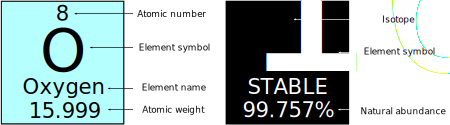
\includegraphics[width=\textwidth]{ElementvsIsotopeSymbol.png}
\end{figure}
The chart of nuclides gives you information about the number protons and neutrons, the 'stability' of the nucleus and in the case of stable isotopes, the natural abundance of each isotope
\end{frame}

\begin{frame}
\frametitle{Different isotopes}
The chart also gives you information about isotope decay, half-life and branching ratios
\begin{figure}
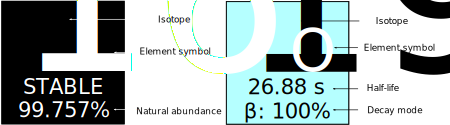
\includegraphics[width=\textwidth]{OxygenIsotopes.png}
\end{figure}
Quick question: How many neutrons does $^{19}$O have?
\end{frame}

\begin{frame}
\frametitle{Different isotopes}
The chart also gives you information about isotope decay, half-life and branching ratios
\begin{figure}
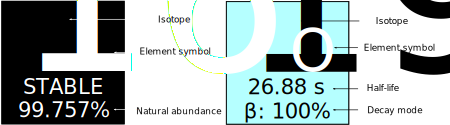
\includegraphics[width=\textwidth]{OxygenIsotopes.png}
\end{figure}
Quick question: How many protons and how many neutrons does $^{19}$O have? \\
\textcolor{blue}{8 protons, 11 neutrons}
\end{frame}

\begin{frame}
\frametitle{Unstable isotopes}
\begin{columns}[c]
\column{0.5\textwidth}
\begin{figure}
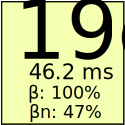
\includegraphics[width=0.7\textwidth]{Carbon19.png}
\end{figure}
\column{0.5\textwidth}
\begin{itemize}
\item 13 neutrons (compared to the 6 neutrons $^{12}$C has)
\item Short half-life (milliseconds)
\item Decays through $\beta$-decay
\item Also decays through $\beta$-delayed neutron emission
\end{itemize}
\end{columns}
\end{frame}

\subsection{Isotopes, isobars and isotones}
\begin{frame}
\frametitle{Nuclear compass}
\begin{columns}
\column{0.5\textwidth}
\begin{figure}
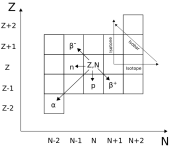
\includegraphics[width=\textwidth]{DecayScheme.png}
\end{figure}
\column{0.5\textwidth}
The positioning of the nuclides along the chart is just as important as the position of the elements on the periodic table.
\vspace{10pt}

Information about decay modes and place in the nuclear landscape.
\end{columns}
\end{frame}


\begin{frame}
\frametitle{Nuclear compass - Isotopes}
\begin{columns}
\column{0.5\textwidth}
\begin{figure}
\includegraphics[width=\textwidth]{DecayScheme-isotope.png}
\end{figure}
\column{0.5\textwidth}
Following the columns, you get isotopes, the same element (proton number) but different neutron numbers
\vspace{10pt} \\
Fun fact: Tin has the largest number of isotopes on the chart
\end{columns}
\end{frame}

\begin{frame}
\frametitle{Nuclear compass - Isotones}
\begin{columns}
\column{0.5\textwidth}
\begin{figure}
\includegraphics[width=\textwidth]{DecayScheme-isotone.png}
\end{figure}
\column{0.5\textwidth}
Following the columns, you get the same neutron number, but different proton numbers
\vspace{10pt} \\
Fun fact: N=82 is the 'most popular' neutron number
\end{columns}
\end{frame}


\begin{frame}
\frametitle{Nuclear compass - Isobars}
\begin{columns}
\column{0.5\textwidth}
\begin{figure}
\includegraphics[width=\textwidth]{DecayScheme-isobar.png}
\end{figure}
\column{0.5\textwidth}
Following the diagonal (right to left), you get isobars: isotopes with the same nucleon number, but different combinations of protons and neutrons \\
\vspace{10pt}
Fun fact: isobars with swapped proton and neutron numbers are called mirror nuclei: \\
\hspace{1pt} $^{34}_{16}$S$_{18}$ and  $^{34}_{18}$Ar$_{16}$
\end{columns}
\end{frame}

\subsection{Trends in the chart}
\begin{frame}
\frametitle{Half-life}
Isotopes decay towards stability
\begin{figure}
\includegraphics[width=0.9\textwidth]{HalfLife+Legend.png}
\end{figure}
\end{frame}

\begin{frame}
\frametitle{Decay Modes}
Distinct regions of decay
\begin{figure}
\includegraphics[width=0.9\textwidth]{DecayMode+Legend.png}
\end{figure}
\end{frame}

%\begin{frame}
%\frametitle{Q$_{\beta^{-}}$}
%A measure of the lik
%\begin{figure}
%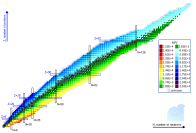
\includegraphics[width=\textwidth]{Qbeta+Legend.png}
%\end{figure}
%\end{frame}

\begin{frame}
\frametitle{Neutron separation energy}
Evidence for magic numbers: how much energy is needed to remove the last neutron from a bound system
\begin{figure}
\includegraphics[width=0.8\textwidth]{Sn+Legend.png}
\end{figure}
\end{frame}

%\begin{frame}
%\frametitle{Q$_{\beta n}$}
%\begin{figure}
%\includegraphics[width=\textwidth]{BetaDelated+legend.png}
%\end{figure}
%\end{frame}

\begin{frame}
\frametitle{Excited states: E$_{2^{+}}$}
Evidence for magic numbers: the energy of the first excited 2$^{+}$ states 
\begin{figure}
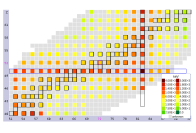
\includegraphics[width=0.9\textwidth]{E2++legend.png}
\end{figure}
\end{frame}

\begin{frame}
\frametitle{NNDC - National Nuclear Data Center}
\href{https://www.nndc.bnl.gov/}{\beamergotobutton{NNDC}}
\begin{figure}
\includegraphics[width=\textwidth]{NNDCScreen.png}
\end{figure}
\end{frame}

\begin{frame}
\frametitle{ENSDF - Evaluated Nuclear Structure File}
\href{https://www.nndc.bnl.gov/ensdf/}{\beamergotobutton{ENSDF}}
\begin{figure}
\includegraphics[width=\textwidth]{ENSDF.png}
\end{figure}
\end{frame}

\section{Applications of isotopic properties}
\subsection{Biology}
\begin{frame}
\frametitle{Nuclear Medicine}
Nuclear properties have become key to treatments:
\begin{columns}[c]
\column{0.5\textwidth}
\begin{figure}
\includegraphics[width=\textwidth]{PET68Ga.png}
Patient with prostrate treated with a $^{225}$Ac compound, imaged with $^{68}$Ga Positron Emission Tomography (PET)
\end{figure}
\column{0.5\textwidth}
\begin{itemize}
\item Specific radiation type
\item Specific half-life and energy
\item Specific chemical properties
\item Development of 'theranostic' pairs
\end{itemize}
\end{columns}
\let\thefootnote\relax\footnote{\tiny{Krotochwil, C. \textit{et al. J. Nuc. Med.} 57 (12) (2016) 1941-1944}}
\end{frame}

\subsection{Materials}
\begin{frame}
\frametitle{Material Science}
\begin{columns}[c]
\column{0.5\textwidth}
Nuclei and nuclear properties can be a useful tool to learn about the world around us. They can provide non-destructive techniques to probe materials. \\
\vspace{10pt}
Neutron radiography can give you complimentary information to an x-ray
\column{0.5\textwidth}
\begin{figure}
\includegraphics[width=0.7\textwidth]{Camera.png}
\end{figure}
\end{columns}
\let\thefootnote\relax\footnote{\tiny{\underline{\textcolor{blue}{\href{https://mnrc.ucdavis.edu/neutron-radiography}{UCDavis - McCellan Nuclear Research Institute}}}}}
\end{frame}

\subsection{Space}
\begin{frame}
\frametitle{Astrophysics}
\begin{columns}[c]
\column{0.5\textwidth}
\begin{figure}
\includegraphics[width=0.8\textwidth]{SolarFlare.jpg}
\end{figure}
\column{0.5\textwidth}
\begin{itemize}
\item The sun burns through fusion: H $\rightarrow$ He
\item As stars evolve, other fusion processes can take over
\item n and p capture are responsible for elements above iron
\item Only possible due to the extreme environments in space
\end{itemize}
Stay tuned: Astrophysics lecture in May
\end{columns}
\let\thefootnote\relax\footnote{\tiny{\underline{\textcolor{blue}{\href{https://www.nasa.gov/content/goddard/nasa-releases-images-of-mid-level-solar-flare/}{NASA - Solar Dynamics Observatory}}}}}
\end{frame}

\begin{frame}
\frametitle{Resources for further reading}
Some light reading:
\begin{itemize}
\item R. A. Dunlap, \textit{An Introduction of to the Physics of Nuclei and Particles}
\item K. Krane, \textit{Introductory Nuclear Physics}
\item W. Loveland \textit{et al.}, \textit{Modern Nuclear Chemistry}
\item G. Friendlander \textit{et al.}, \textit{Nuclear and Radiochemistry}
\item C. A. Bertulani, \textit{Nuclear Physics in a Nutshell}
\end{itemize}
Some advanced reading:
\begin{itemize}
\item K. Heyde, \textit{Basic Ideas and Concepts in Nuclear Physics}
\end{itemize}
Some fun reading:
\begin{itemize}
\item P. Bizony, \textit{Atom}
\end{itemize}
\end{frame}
 


\end{document} 


